% A FAIRE
% Lier au thème de la ville
% Enoncer un but
% Montrer exemples (1 à 2) -> motivation
% Enoncer limitations (théo Rice -> côté ENS faire la preuve). Donc impossible de le vérifier à coup sûr dans le cas général.
% Solution: interprétation abstraite. Présentation vite fait de quelques moyens existant sur les strings.
% Moi, je fais mon propre "domaine d'interprétation abstrait": les automates.
% Explication rapide de comment ça se passe (on récupère l'ens. des états possibles au fur et à mesure puis inclus dans auto de ref).
% Je voulais le faire sur les grammaires, mais pb d'inclusion d'une grammaire dans un autre -> indécidable. Donc limité automates.

% 1ère partie: mise en place des outils.
% structure de représentation choisie (en OCAML): a = {...}, hashmap de transition. J'ai créé une lib entière pour.
% on peut donc construire toutes les opérations usuelles des automates là-dessus (union, inters, concat)
% ensuite, on crée un petit langage sur lequel je peux lancer tout ça.
% On se limite à 3 primitives pour simplifier: assignation string, concat, input utilisateur.
% On présente ici 2 quelques manières par lesquelles on construit l'automate: assignation directe, if/else, while.

% 2ème partie: application du modèle.
% On fait dérouler un programme en direct pour le montrer en application. (AST / prog clair / graphviz à chaque étape)
% On remarque qu'alors on arrive à montrer les modulo 3 et autres exemples d'applications.
% Screenshot du code qui marche. (TODO)

% Dernière partie: Amélioration du modèle. (TODO)
% Motivation: exemple du 2^n états des if/else consécutifs.
% On se concentre alors sur la réduction. D'ABORD JE FAIS LES TRUCS AVANT HEIN
% Résultats: mémoire + temps d'exec pour bcp bcp de if/else avec/sans réduction. Établir limite à laquelle c'est utile.
% Showcase de 2eme algo pour comparer. Tableaux récapitulatifs. (même diagramme évolution ?)
% Profiler pour voir quelles fonctions sont les + coûteuses...

% CCL pk pas des grammaires/automates à piles ? Pcq inclusion indécidable.
% Annexe preuve th. de Rice


\documentclass{beamer}
\usepackage{listings}
\usepackage{graphicx}
\graphicspath{ {./images/} }

\usetheme{Madrid}

%Information inclue dans la page de présentation
\title{Vérification automatique de la correction de strings formés dynamiquement}
\subtitle{TIPE}
\author{Maire Grégoire}
\date{2023}

% Met la table des matières au début de chaque section
\AtBeginSection[]
{
  \begin{frame}
    \frametitle{Table des matières}
    \tableofcontents[currentsection]
  \end{frame}
}


%--------------------------------------------------------------
% Début du document
\begin{document}

\frame{\titlepage}

\begin{frame}
  \frametitle{Motivations}
  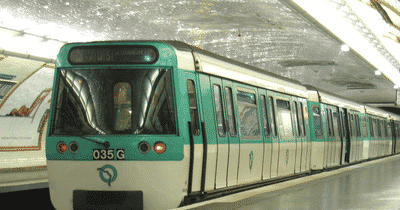
\includegraphics{ img_metro }
  % 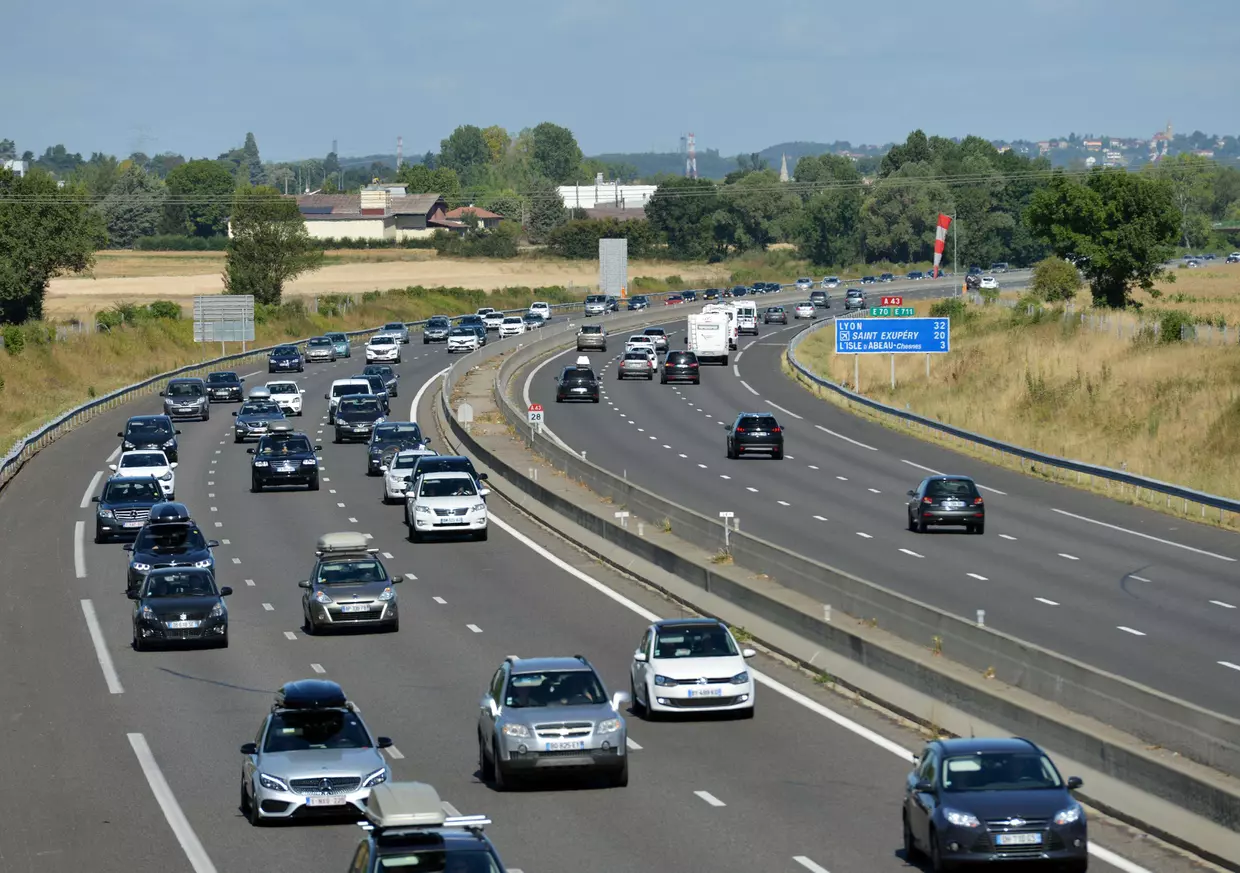
\includegraphics{ img_autoroute }
  \begin{itemize}
    \item En ville, les métros, voiture, avions ou autres transports en commun
      nécessitent l'assurance que leurs programmes soient corrects
    \item Longs programmes : besoin de preuves automatisées
    \item Mon but: automatiser les preuves d'invariants sur les strings dans les programmes
  \end{itemize}
\end{frame}

\begin{frame}
  \frametitle{Motivations}
  Plus précisément, mon intérêt : construction dynamique d'un string dans un programme. \\
  Exemple d'application:
  \begin{itemize}
    \item Vérification d'un message d'urgence formatté d'un métro à une unité de contrôle
  \end{itemize}
  
\end{frame}

\begin{frame}
  \frametitle{Limitation}
  Ce qu'on aurait envie de faire : récolter l'ensemble des états possibles d'un string
  à la fin du code d'un programme. Mais ce n'est pas toujours possible :
  \begin{alertblock}{Limitation : Théorème de Rice}
  Toute propriété sémantique non triviale d'un programme est indécidable (impossible à vérifier automatiquement).
  \end{alertblock}
  \begin{itemize}
    \item D'où l'utilisation d'une méthode pour contourner la limitation :
      "l'interprétation abstraite", consistant en une sur-approximation des états possibles d'arrivée. \\
    \item Toujours possible de sur-approximer.
    \item Peut mener à des faux-négatifs, mais jamais à des faux-positifs. Mathématiquement correct !
  \end{itemize}
\end{frame}

\begin{frame}
  \frametitle{Choix d'un domaine abstrait}
  Pour ce faire, on définit un "domaine abstrait" qui permettra de
  représenter l'ensemble des valeurs prises par le string, (un
  ensembles de strings) sans les énumérer 1 par 1, qui soit numériquement représentable
  (car il arrive qu'on doive représenter des infinités de strings). \\
  
  Divers autheurs se sont déjà penché sur ce problème, avec des domaines tels que:
  \begin{itemize}
    \item Domaine sur les préfixes : "l'ensemble de tous les strings commençant par..."
    \item Domaine sur les facteurs communs: "l'ensemble de tous les strings ayant comme facteur..."
  \end{itemize}
  
  J'ai choisi un domaine encore inexploré : la représentation par automates.
  \begin{itemize}
    \item[\textcolor{green}{\textbullet}] Précis dans ce qu'ils représentent (ensemble des langages rationnels)
    \item[\textcolor{red}{\textbullet}] + coûteux en calculs
  \end{itemize}
\end{frame}

\begin{frame}
  \frametitle{Un exemple motivant}
  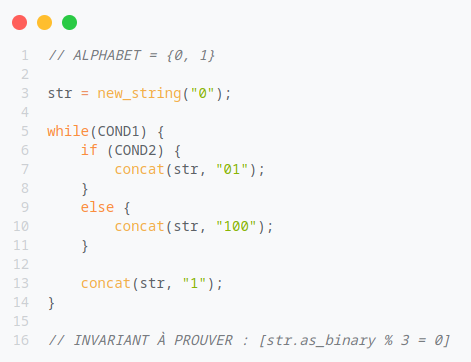
\includegraphics[scale=0.7]{ prog0 } \\ % TODO refaire image
  Un programme construisant des nombres congru à 0 modulo 3. Prouvons sa correction automatiquement !
\end{frame}

\begin{frame}
  \frametitle{Table of Contents}
  \tableofcontents
\end{frame}

\section{Mise en place des outils}

\begin{frame}
  \frametitle{Structure d'automates}
  
\end{frame}


\section{Application du modèle}


\begin{frame}
  \frametitle{Structure d'automates}
  blank
\end{frame}

\section{Améliorations diverses}

\begin{frame}
  \frametitle{Explosion d'états} % comparer 2 approches (déterminiser à l'avance, ou non) + graphiques comparatif
  blank
\end{frame}

\end{document}

